\chapter{Zadanie projektowe}

Zadaniem projektowym tej części naszej pracy było przygotowanie oraz dobranie optymalnych nastawów regulatorów w środowisku Matlab. W części a) należało dobrać strukturę i nastawy dwupętlowego układu regulacji PI/PID z odsprzęganiem i bez odsprzęgania. Kolejno, należało zaprojektować i zaimplementować analityczny regulator predykcyjny z uwzględnieniem ograniczeń przez rzutowanie oraz, w części c), numeryczny regulator predykcyjny z uwzględnieniem ograniczeń na sterowanie. Następnie należało porównać działanie tych regulatorów.
\\\\ Algorymem regulatora jaki należało zaimplementować w części b) i c) w ramach naszego zadania był regulator predykcyjny DMC (Dynamic Matrix Control)\\\\

Regulator DMC


\begin{figure}[h!]
	\centering
	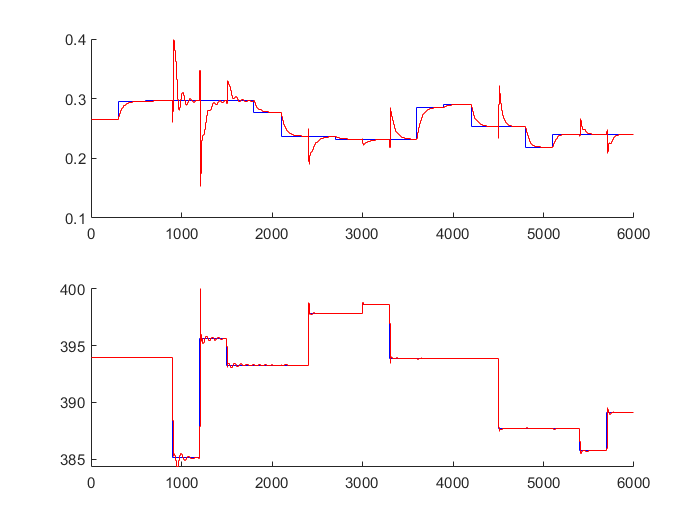
\includegraphics[width=.6\linewidth]{img/yDMC.png}
	\label{ch2:regulator}
	\caption{Regulacja DMC analityczna - wyjście na tle wartości zadanej}
\end{figure}

\begin{figure}[h!]
	\centering
	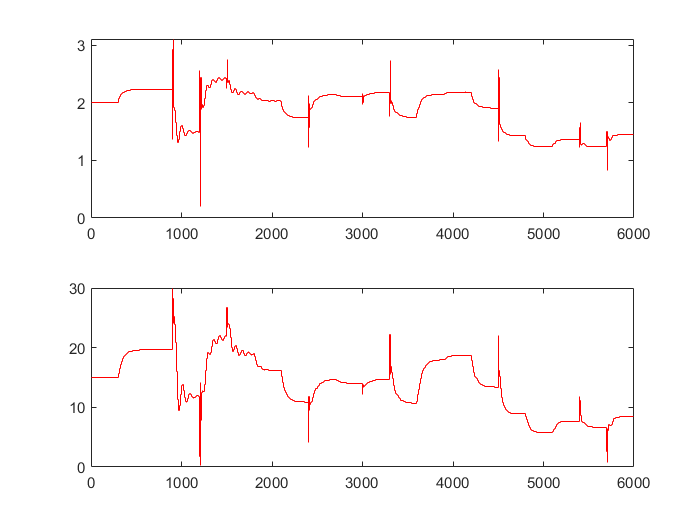
\includegraphics[width=.6\linewidth]{img/uDMC.png}
	\label{ch2:regulator}
	\caption{Regulacja DMC analityczna - sterowanie}
\end{figure}



\begin{figure}[h!]
	\centering
	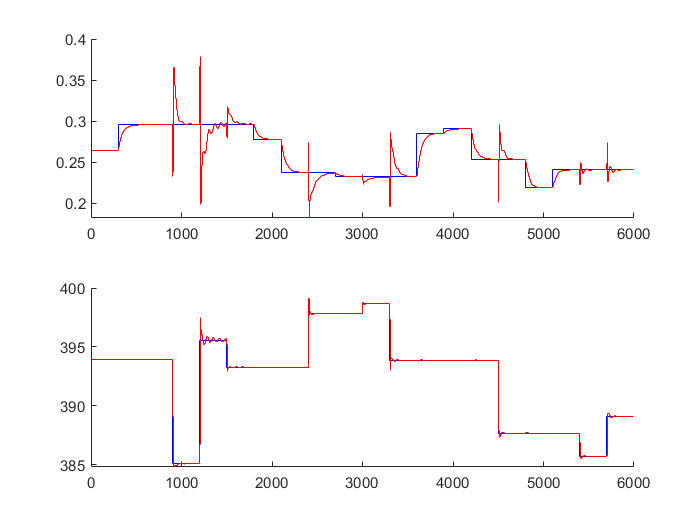
\includegraphics[width=.6\linewidth]{img/yDMCnum.png}
	\label{ch2:regulator}
	\caption{Regulacja DMC numeryczna - wyjście na tle wartości zadanej}
\end{figure}

\begin{figure}[h!]
	\centering
	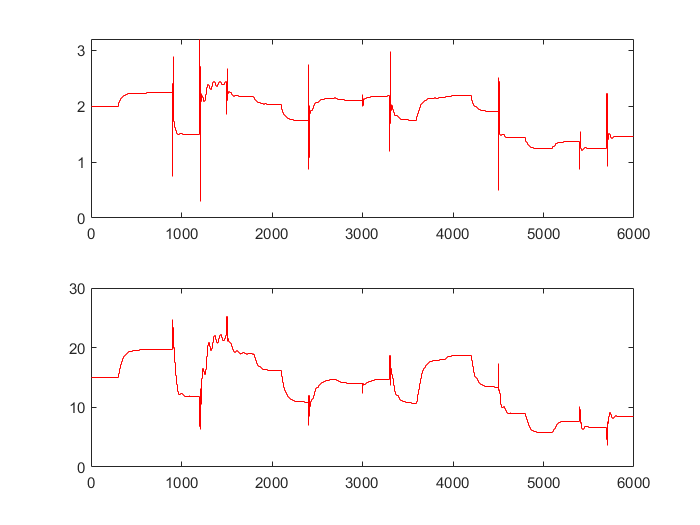
\includegraphics[width=.6\linewidth]{img/uDMCnum.png}
	\label{ch2:regulator}
	\caption{Regulacja DMC numeryczna - sterowanie}
\end{figure}
